\documentclass[aspectratio=169]{beamer}
\mode<presentation>
{
  \usetheme{metropolis}      % or try Darmstadt, Madrid, Warsaw, ...
  \usecolortheme{default} % or try albatross, beaver, crane, ...
  \usefonttheme{structurebold}  % or try serif, structurebold, ...
  \setbeamercolor{background canvas}{bg=white}
  \setbeamertemplate{navigation symbols}{}
  \setbeamertemplate{bibliography item}{\insertbiblabel}
  %\setbeamertemplate{caption}[numbered]
} 
\usepackage[english]{babel}
\usepackage[utf8x]{inputenc}
\usepackage{listings}             % Include the listings-package
\hypersetup{
    colorlinks = true,
    linkcolor = {black},
    urlcolor = {blue}
}
\usepackage{animate}
\usepackage{bm}

\setbeamertemplate{caption}{\raggedright\insertcaption\par}


\DeclareMathOperator*{\argmin}{arg\,min}

\title[Deep Learning and Temporal Data Processing]{Deep Learning and Temporal Data Processing}
\subtitle{0 - Gradient Descent}
\institute{University of Modena and Reggio Emilia}
\author{Andrea Palazzi}
\date{July 10th, 2017}

\def\thisframelogos{}

\newcommand{\framelogo}[1]{\def\thisframelogos{#1}}

\addtobeamertemplate{frametitle}{}{%
\begin{tikzpicture}[remember picture,overlay]
\node[anchor=north east] at (current page.north east) {%
    \foreach \img in \thisframelogos {%
        %\hspace{.5ex}%
        \includegraphics[height=3.5ex]{\img}%
    }%
};
\end{tikzpicture}}

\begin{document}

\framelogo{img/template/logo_unimore_white.png}

\bgroup
\renewcommand{\insertframenumber}{}
\begin{frame}[noframenumbering]
  \titlepage
\end{frame}
\egroup
\begin{frame}{Agenda}
  \tableofcontents
\end{frame}



%%%%%%%%%%%%%%%%%%%%%%%%%%%%%%%%%%%%%%%%%%%%%%%%%%%%%%%%%%%%%%%%%%
%%%%%%%%%%%%%%%%%%%%%%%%%%%%%%%%%%%%%%%%%%%%%%%%%%%%%%%%%%%%%%%%%%
%%%%%%%%%%%%%%%%%%%%%%%%%%%%%%%%%%%%%%%%%%%%%%%%%%%%%%%%%%%%%%%%%%


\section{Gradient Descent}

\begin{frame}{Gradient Descent}
\textbf{Gradient descent} is an iterative optimization algorithm for finding the minimum of a function. How? Take step proportional to the negative of the gradient of the function at the current point.
\begin{figure}
\begin{tabular}{c}
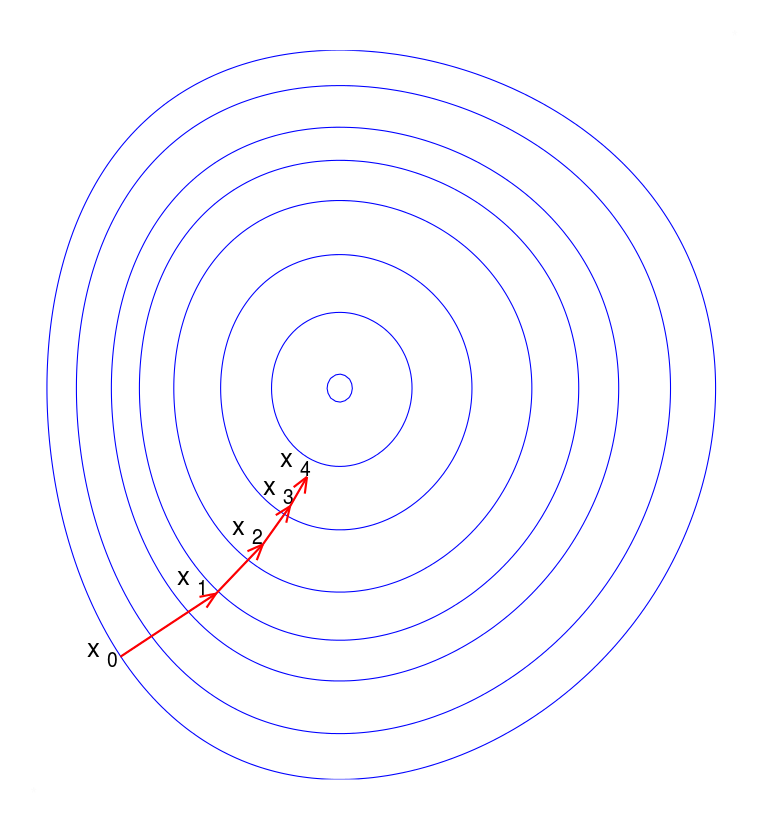
\includegraphics[width=0.3\textwidth]{img/sgd/level_sets.png}
\end{tabular}
\caption{Gradient descent on a series of level sets}
\end{figure}
\end{frame}

\begin{frame}{Gradient Descent Update}
If we consider a function $f(\bm{\theta})$, the \textbf{gradient descent update} can be expressed as:
\begin{equation}
\theta_j := \theta_j - \alpha \frac{\partial}{\partial \theta_j} f(\bm{\theta})
\end{equation}
for each parameter $\theta_j$.\\
\vspace{0.5cm}
The size of the step is controlled by \textbf{learning rate} $\alpha$.
\end{frame}

%%%%%%%%%%%%%%%%%%%%%%%%%%%%%%%%%%%%%%%%%%%%%%%%%%%%%%%%%%%%%%%%%%

%%%%%%%%%%%%%%%%%%%%%%%%%%%%%%%%%%%%%%%%%%%%%%%%%%%%%%%%%%%%%%%%%%

\begin{frame}{Visualizing Gradient Descent}
\begin{figure}
\begin{tabular}{c}
Gradient Descent for 1-d function $f(\theta)$.\\
  \animategraphics[loop,controls,width=0.9\textwidth]{1}{img/sgd/descent/descent-}{0}{7}
\end{tabular}
\end{figure}
\end{frame}


%%%%%%%%%%%%%%%%%%%%%%%%%%%%%%%%%%%%%%%%%%%%%%%%%%%%%%%%%%%%%%%%%%

\begin{frame}{Convexity}
Turns out that if the function is \textbf{convex} gradient descent will converge to the \textbf{global minimum}. For \textbf{non-convex} functions, it may converge to \textbf{local minima}.
\begin{figure}
\begin{tabular}{cc}
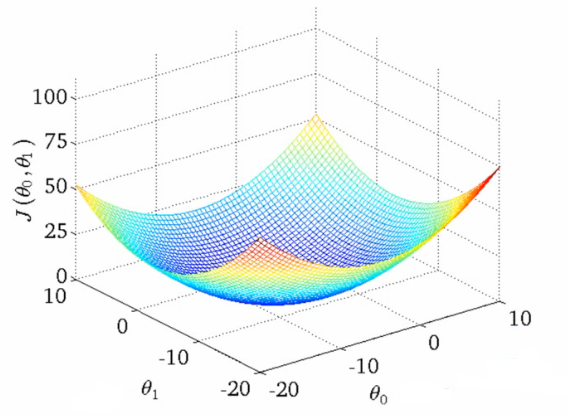
\includegraphics[width=0.4\textwidth]{img/sgd/convex_function.png} &
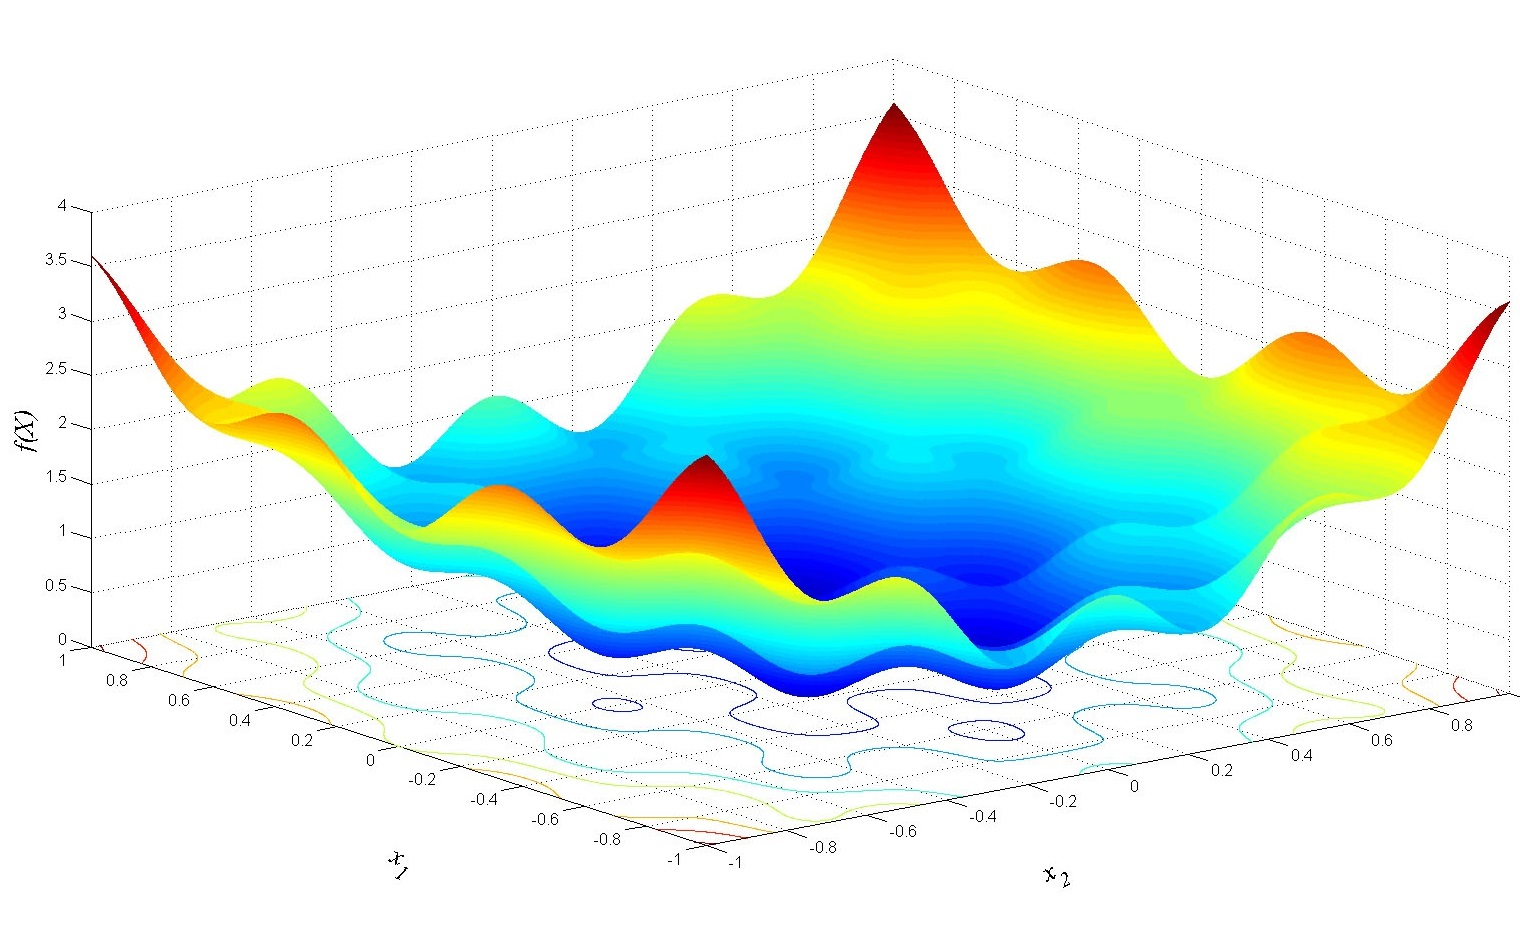
\includegraphics[width=0.4\textwidth]{img/sgd/non_convex_function.jpg}\\
Convex Function & Non-Convex Function
\end{tabular}
\end{figure}
\end{frame}

%%%%%%%%%%%%%%%%%%%%%%%%%%%%%%%%%%%%%%%%%%%%%%%%%%%%%%%%%%%%%%%%%%

\begin{frame}{Gradient Descent}
Gradient descent is often used in machine learning to \textbf{minimize a cost function}, usually also called \textit{objective} or \textit{loss} function and denoted $L(\cdot)$ or $J(\cdot)$.\\
\vspace{0.5cm}
The cost function depends on the model's parameters and is a proxy to evaluate model's performance. Generally speaking, in this framework minimizing the cost equals to maximizing the effectiveness of the model.

\end{frame}

%%%%%%%%%%%%%%%%%%%%%%%%%%%%%%%%%%%%%%%%%%%%%%%%%%%%%%%%%%%%%%%%%%

\begin{frame}{Stochastic Gradient Descent}
In principle, to perform a single update step you should run through all your training examples. This is known as \textbf{batch gradient descent}.\\
\vspace{0.5cm}
A different strategy is the one of \textbf{minibatch stochastic gradient descent}. In this case, only a small subset of the training dataset is considered at each update step.\\
\vspace{0.5cm}
In the extreme case in which only a random example of the training set is considered to perform the update step, we talk of \textbf{stochastic gradient descent}.

\end{frame}

%%%%%%%%%%%%%%%%%%%%%%%%%%%%%%%%%%%%%%%%%%%%%%%%%%%%%%%%%%%%%%%%%%

\begin{frame}{Learning Rate}
Choosing the the right \textbf{learning rate} $\bm{\alpha}$ is essential to correctly proceed towards the minimum. A step \textit{too small} could lead to an extremely \textit{slow} convergence. If the step is \textit{too big} the optimizer could \textit{overshoot} the minimum or even \textit{diverge}. 
\begin{figure}
\begin{tabular}{ccc}
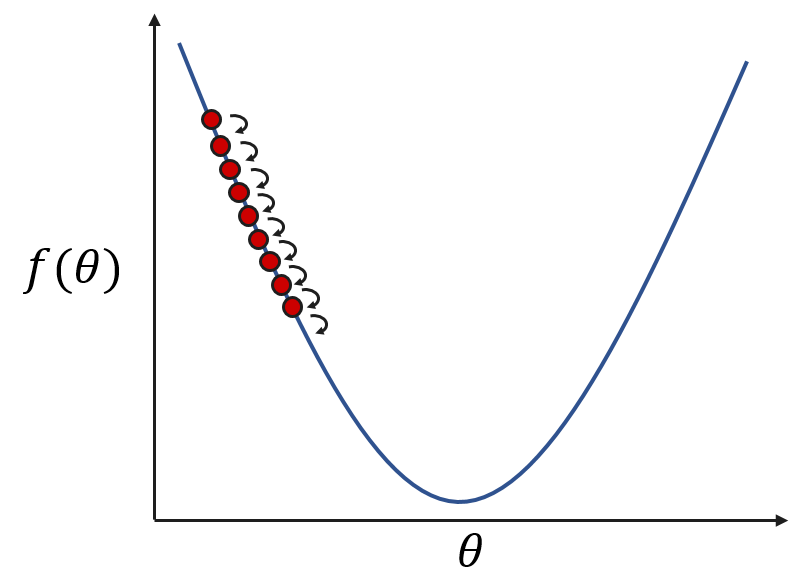
\includegraphics[width=0.35\textwidth]{img/sgd/lr_too_small.png} &
\quad &
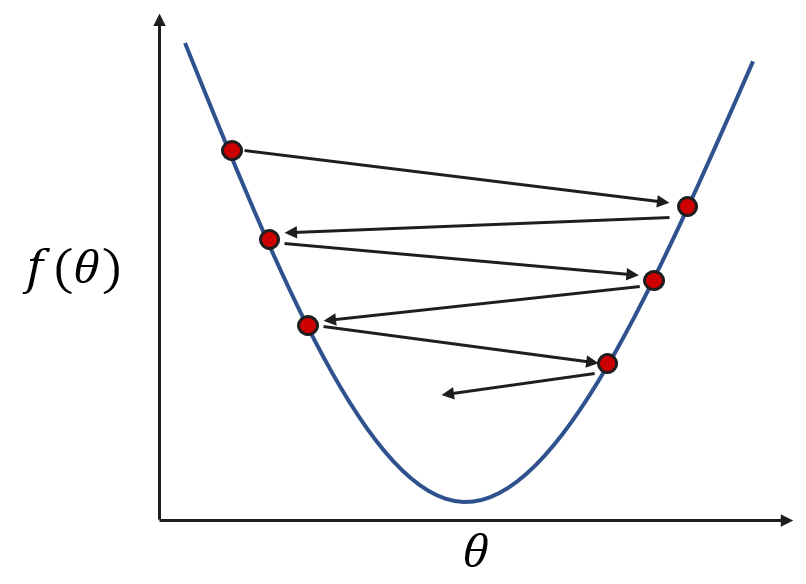
\includegraphics[width=0.35\textwidth]{img/sgd/lr_too_big.png}\\
Learning Rate too small & & Learning Rate too big
\end{tabular}
\end{figure}

\end{frame}

%%%%%%%%%%%%%%%%%%%%%%%%%%%%%%%%%%%%%%%%%%%%%%%%%%%%%%%%%%%%%%%%%%

\begin{frame}{Advanced Optimizers}
In practice, it's quite rare to see the procedure described above (so called \textbf{vanilla SGD}) used for optimization in the real-world.\\
\vspace{0.5cm}
Conversely, a number of cutting-edge optimizers  \cite{kingma2014adam,duchi2011adaptive,zeiler2012adadelta} are commonly used. However, these advanced optimization techniques are out of the scope of this short overview.
\end{frame}

%%%%%%%%%%%%%%%%%%%%%%%%%%%%%%%%%%%%%%%%%%%%%%%%%%%%%%%%%%%%%%%%%%
%%%%%%%%%%%%%%%%%%%%%%%%%%%%%%%%%%%%%%%%%%%%%%%%%%%%%%%%%%%%%%%%%%
%%%%%%%%%%%%%%%%%%%%%%%%%%%%%%%%%%%%%%%%%%%%%%%%%%%%%%%%%%%%%%%%%%

\section{Credits}
\begin{frame}[t, allowframebreaks]{Credits}
These slides heavily borrow from a number of awesome sources. I'm really grateful to all the people who take the time to share their knowledge on this subject with others.\\
\vspace{0.5cm}
In particular:
\begin{itemize}
\item Stanford CS231n Convolutional Neural Networks for Visual Recognition\\
\url{http://cs231n.stanford.edu/}
\item Stanford CS20SI TensorFlow for Deep Learning Research\\
\url{http://web.stanford.edu/class/cs20si/syllabus.html}
\item Deep Learning Book (GoodFellow, Bengio, Courville)\\
\url{http://www.deeplearningbook.org/}
\item Marc'Aurelio Ranzato, "Large-Scale Visual Recognition with Deep Learning"\\
\url{www.cs.toronto.edu/~ranzato/publications/ranzato_cvpr13.pdf}
\item Convolution arithmetic animations\\
\url{https://github.com/vdumoulin/conv_arithmetic}
\item Andrej Karphathy personal blog\\
\url{http://karpathy.github.io/}
\item WildML blog on AI, DL and NLP\\
\url{http://www.wildml.com/}
\item Michael Nielsen Deep Learning online book
\url{http://neuralnetworksanddeeplearning.com/}
\end{itemize}
\end{frame}

%%%%%%%%%%%%%%%%%%%%%%%%%%%%%%%%%%%%%%%%%%%%%%%%%%%%%%%%%%%%%%%%%%
%%%%%%%%%%%%%%%%%%%%%%%%%%%%%%%%%%%%%%%%%%%%%%%%%%%%%%%%%%%%%%%%%%
%%%%%%%%%%%%%%%%%%%%%%%%%%%%%%%%%%%%%%%%%%%%%%%%%%%%%%%%%%%%%%%%%%

\section{References}

\begin{frame}[t, allowframebreaks]
\frametitle{References}
\bibliographystyle{abbrv}
\bibliography{bibliography}
\end{frame}
\end{document}